\documentclass[12pt,a4paper]{article}
\usepackage[utf8]{inputenc}
\usepackage[brazilian]{babel}
\usepackage{amsmath}
\usepackage{amsfonts}
\usepackage{amssymb}
\usepackage[T1]{fontenc}
\usepackage{graphicx}
\usepackage{physics}
\usepackage{siunitx}
\newcounter{prob}
\newcounter{subprob}
\renewcommand{\thesubprob}{\alph{subprob}}

\newcommand{\problem}{\setcounter{subprob}{0} \stepcounter{prob} \par \medskip \noindent \textbf{Problema~\theprob \ }}

\newcommand{\answer}{\par \medskip \noindent \textit{Resposta \ }}

\newcommand{\finalanswer}[1]{
	\begin{center} 
    	{\renewcommand{\arraystretch}{1.5}
		\renewcommand{\tabcolsep}{0.2cm} 
    	\begin{tabular}{|c|} 
    		\hline 
        	$ \displaystyle #1 $  \\ 
        	\hline 
    	\end{tabular}} 
   	\end{center}}

\newcommand{\subproblem}{\stepcounter{subprob} \par \smallskip \noindent \quad \textit{(\thesubprob) \ }}

\newcommand{\subanswer}{\par \smallskip \noindent \quad \textit{Resposta \ }}

\newcommand{\option}{\item[$\square$]}
\newcommand{\thisone}{\item[$\blacksquare$]}

\newenvironment{subitemize}{\begin{itemize}}{\end{itemize}}

\author{Aluno - Código do Aluno}
\title{Lista de Exercícios - Código da Disciplina}
\date{}
\begin{document}

%%--CABEÇALHO--%%
	\begin{center}
    {\large Lista de Exercícios I\par (Sinais e sistemas) \par}
    {\large Processamento Digital de Sinais\par}
    {\large Engenharia de Telecomunicações \par}
   % {\large Prof. André L. F. de Almeida \par}
	\end{center}

\begin{center}
   INSTRUÇÕES
\end{center} 
\begin{subitemize}
 %   \option Não
    \thisone A lista deve ser enviada para o instrutor de apoio da disciplina.
    \thisone A lista deve ser feita de próprio punho não podendo, portanto, fazer uso de editores de texto.
    \thisone  As listas deverão ser enviadas  no formato pdf legível.
    \thisone Na solução, o aluno deve apresentar o desenvolvimento matemático em detalhes para todas soluções.
   % \option Talvez
\end{subitemize}
\problem Um sistema LIT causal tem a seguinte função de sistema:
\begin{equation}
    H(Z) = \dfrac{4 + 0,25z^{-1} - 0,5z^{-2}}{\left(1 - 0,25z^{-1} \right)\left(1 + 0,5z^{-1} \right)}
\end{equation}
\subproblem Qual é a RDC para $H(Z)$?
\subproblem Determine se o sistema é estável ou não.
\subproblem Determine a equação de diferenças que é satisfeita
pela entrada $x[n]$ e pela saída $y[n]$.
\subproblem Use a expansão em frações parciais para determinar
a resposta ao impulso $h[n]$.
\subproblem Encontre $Y(Z)$, a transformada $Z$ da saída, quando
a entrada é $x[n]~ = u[-n-1]$. Especificar a RDC
para $Y(z)$.
\subproblem Encontre a sequência de saída $y[n]$ quando a entrada
é $x[n] = u[-n-1]$.

\answer 

\problem Determine a resposta ao degrau unitário do sistema causal
para o qual a transformada $Z$ da resposta ao impulso é
\begin{equation}
    H(Z) = \dfrac{1 - z^3}{1 - z^4}
\end{equation}
	
\answer

\problem Se a entrada $x[n]$ de um sistema LIT for $x[n] = u[n]$, a saída é
\begin{equation}
    y[n] = \left( \dfrac{1}{2} \right)^{n-1}u[n + 1]
\end{equation}
\subproblem Determine $H(z)$, a transformada $z$ da resposta ao impulso
do sistema, e esboce seu diagrama de polos e zeros.
\subproblem Encontre a resposta ao impulso $h[n]$.
\subproblem O sistema é estável?
\subproblem O sistema é causal?

\answer

\problem Considere uma sequência $x[n]$ para a qual a transformada
$z$ é
\begin{equation}
    X(Z) = \dfrac{\dfrac{1}{3}}{1 - \dfrac{1}{2}z^{-1}} + \dfrac{\dfrac{1}{4}}{1 - 2z^{-1}}
\end{equation}
e para a qual a RDC inclui a circunferência unitária. Determine
$x[0]$ usando o teorema do valor inicial.

\answer

\problem Usando uma expansão em série de potência determine a sequência $x[n]$ cuja transformada $Z$ é
\begin{equation}
X(Z) = e^{z}    
\end{equation}

\answer

\problem Considere um sistema LIT que seja estável e para o
qual $H(Z)$, a transformada $Z$ da resposta ao impulso,
seja dada por
\begin{equation}
    H(Z) = \dfrac{3}{1 - \dfrac{1}{3}z^{-1}}
\end{equation}
Suponha que $x[n]$, a entrada do sistema, seja uma sequência
degrau unitário.
\subproblem Determine a saída $y[n]$ calculando a convolução
discreta de $x[n]$ e $h[n]$.
\subproblem Determine a saída $y[n]$ calculando a transformada
$Z$ inversa de $Y(Z)$.

\answer

\problem Seja x[n] a sequência com o diagrama de polos e zeros
mostrado na Figura \ref{fig7}. Esboce o diagrama de polos e zeros para:

\begin{equation}
    y[n] = \left(\dfrac{1}{2}\right)^n x[n]
\end{equation}
\begin{figure}[h!]
    \centering
    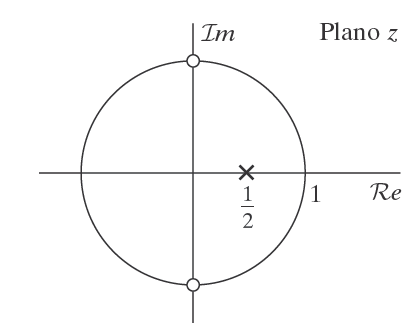
\includegraphics[scale=0.6]{Fig/fig7.png}
    \caption{Figura para solução do problema 7}
    \label{fig7}
\end{figure}

\answer

\problem O diagrama de polos e zeros na Figura \ref{fig8} corresponde
à transformada $Z$ $X(Z)$ de uma sequência causal $x[n]$. Esboce
o diagrama de polos e zeros de $Y(Z)$, em que $y[n] = x[-n + 3]$. Além disso, especifique a RDC para $Y(Z)$.
\begin{figure}[h!]
    \centering
    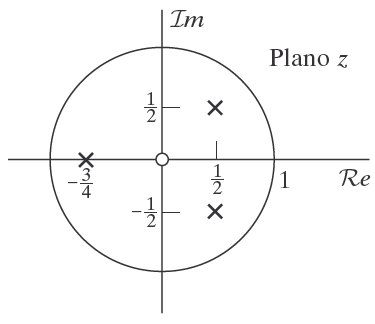
\includegraphics[scale=0.6]{Fig/feg8.png}
    \caption{Figura para solução do problema 8}
    \label{fig8}
\end{figure}

\answer

\problem Considere a transformada $Z$ $X(Z)$, cujo diagrama de polos
e zeros é como mostrado na Figura \ref{fig9}. 
\subproblem Determine a RDC de $X(Z)$ se sabemos que a transformada
de Fourier existe. Para esse caso, determine se a sequência $x[n]$ correspondente é lateral direita, lateral esquerda ou bilateral.
\subproblem Quantas possíveis sequências bilaterais tem o diagrama de polos e zeros mostrado na Figura \ref{fig9}?
\subproblem É possível que o diagrama de polos e zeros na Figura \ref{fig9} seja associado com uma sequência que é tanto estável quanto causal? Nesse caso, dê a RDC apropriada.

\begin{figure}[h!]
    \centering
    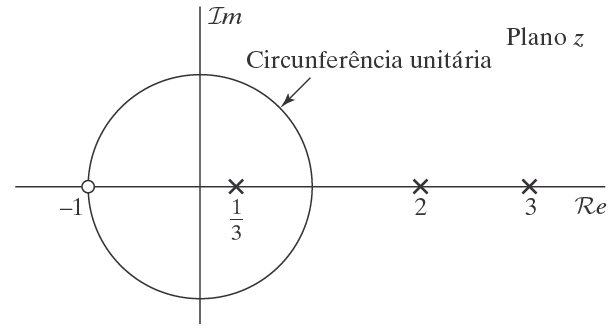
\includegraphics[scale=0.6]{Fig/fig9.png}
    \caption{Figura para solução do problema 9}
    \label{fig9}
\end{figure}

\problem Para o par de transformadas $Z$ da
entrada e da saída $X(Z)$ e $Y(Z)$, determine a RDC para a função de sistema $H(Z)$:
 \begin{equation*}
\begin{split}
    &X(Z) = \dfrac{1}{1 - \dfrac{3}{4}z^{-1}}\; , |z| > \dfrac{3}{4}\\
    &Y(Z) = \dfrac{1}{1 + \dfrac{2}{3}z^{-1}}\; , |z| > \dfrac{2}{3}
\end{split}
\end{equation*}

%\begin{subitemize}
 %   \option Não
  %  \thisone Sim
   % \option Talvez
%\end{subitemize}

\end{document}
